\begin{figure}[!htbp]
\centering
\begin{tikzpicture}[schema base]
\node[schema titolo] at (0,1) {Esperimento: 10 compiti, 5 coppie di difficoltà simile};
\foreach \coppia in {1,2,3,4,5} {
  \begin{scope}[shift={({0.25+3*(\coppia-1)},0)}]
    \path[schema pannello,fill=schemaCartaGialla!50] (0,-0.7) rectangle (2.65,0.4);
    \node[draw=schemaVerde,fill=schemaCartaVerde,inner sep=4pt] at (0.68,-0.12) {\coppia A};
    \node[draw=schemaBlu,fill=schemaCartaBlu,inner sep=4pt] at (1.95,-0.12) {\coppia B};
  \end{scope}
}
\node[schema pannello,fill=schemaGrigio!3,minimum width=8cm,minimum height=1.9cm,inner sep=0pt] (partecipante) at (7.5,-2.15) {};
\pic[scale=0.95] at (5.15,-2.15) {persona};
\node[schema etichetta,text width=4.5cm] at (9,-2.15) {Lo stesso partecipante\\usa entrambe le condizioni};
\draw[schema freccia] (7.5,-0.85) -- (partecipante.north);
\path[schema pannello,draw=schemaVerde,fill=schemaCartaVerde!35] (0,-3.65) rectangle (6.6,-7.4);
\path[schema pannello,draw=schemaBlu,fill=schemaCartaBlu!50] (8.4,-3.65) rectangle (15,-7.4);
\node[schema titolo] at (0.3,-4.05) {A\quad Assistente AI};
\node[schema titolo] at (8.7,-4.05) {B\quad Consultazione del manuale};
\coordinate (biforcazione) at (7.5,-3.32);
\draw[schema freccia,-] (partecipante.south) -- (biforcazione);
\draw[schema freccia,rounded corners=2pt,-{Straight Barb[length=2mm,width=2mm]}] (biforcazione) -| (3.3,-3.65);
\draw[schema freccia,rounded corners=2pt,-{Straight Barb[length=2mm,width=2mm]}] (biforcazione) -| (11.7,-3.65);
\node[draw=schemaVerde,fill=white,rounded corners=4pt,text width=3.5cm,align=center,inner sep=4pt,font=\schemafont\footnotesize] (domanda) at (2.35,-4.95) {Domanda\\dell'operatore};
\node[draw=schemaVerde,fill=white,rounded corners=4pt,text width=3.5cm,align=center,inner sep=4pt,font=\schemafont\footnotesize,below=3mm of domanda] (risposta) {Risposta dal testo\\del manuale};
\draw[schema freccia,draw=schemaVerde,-{Straight Barb[length=1.4mm,width=1.4mm]}] (domanda.south) -- (risposta.north);
\pic[scale=0.55] at (5.3,-5.45) {modello};
\node[schema etichetta] at (3.3,-6.95) {RAG locale con Qwen3-4B text-only};
\node at (9.9,-5.55) {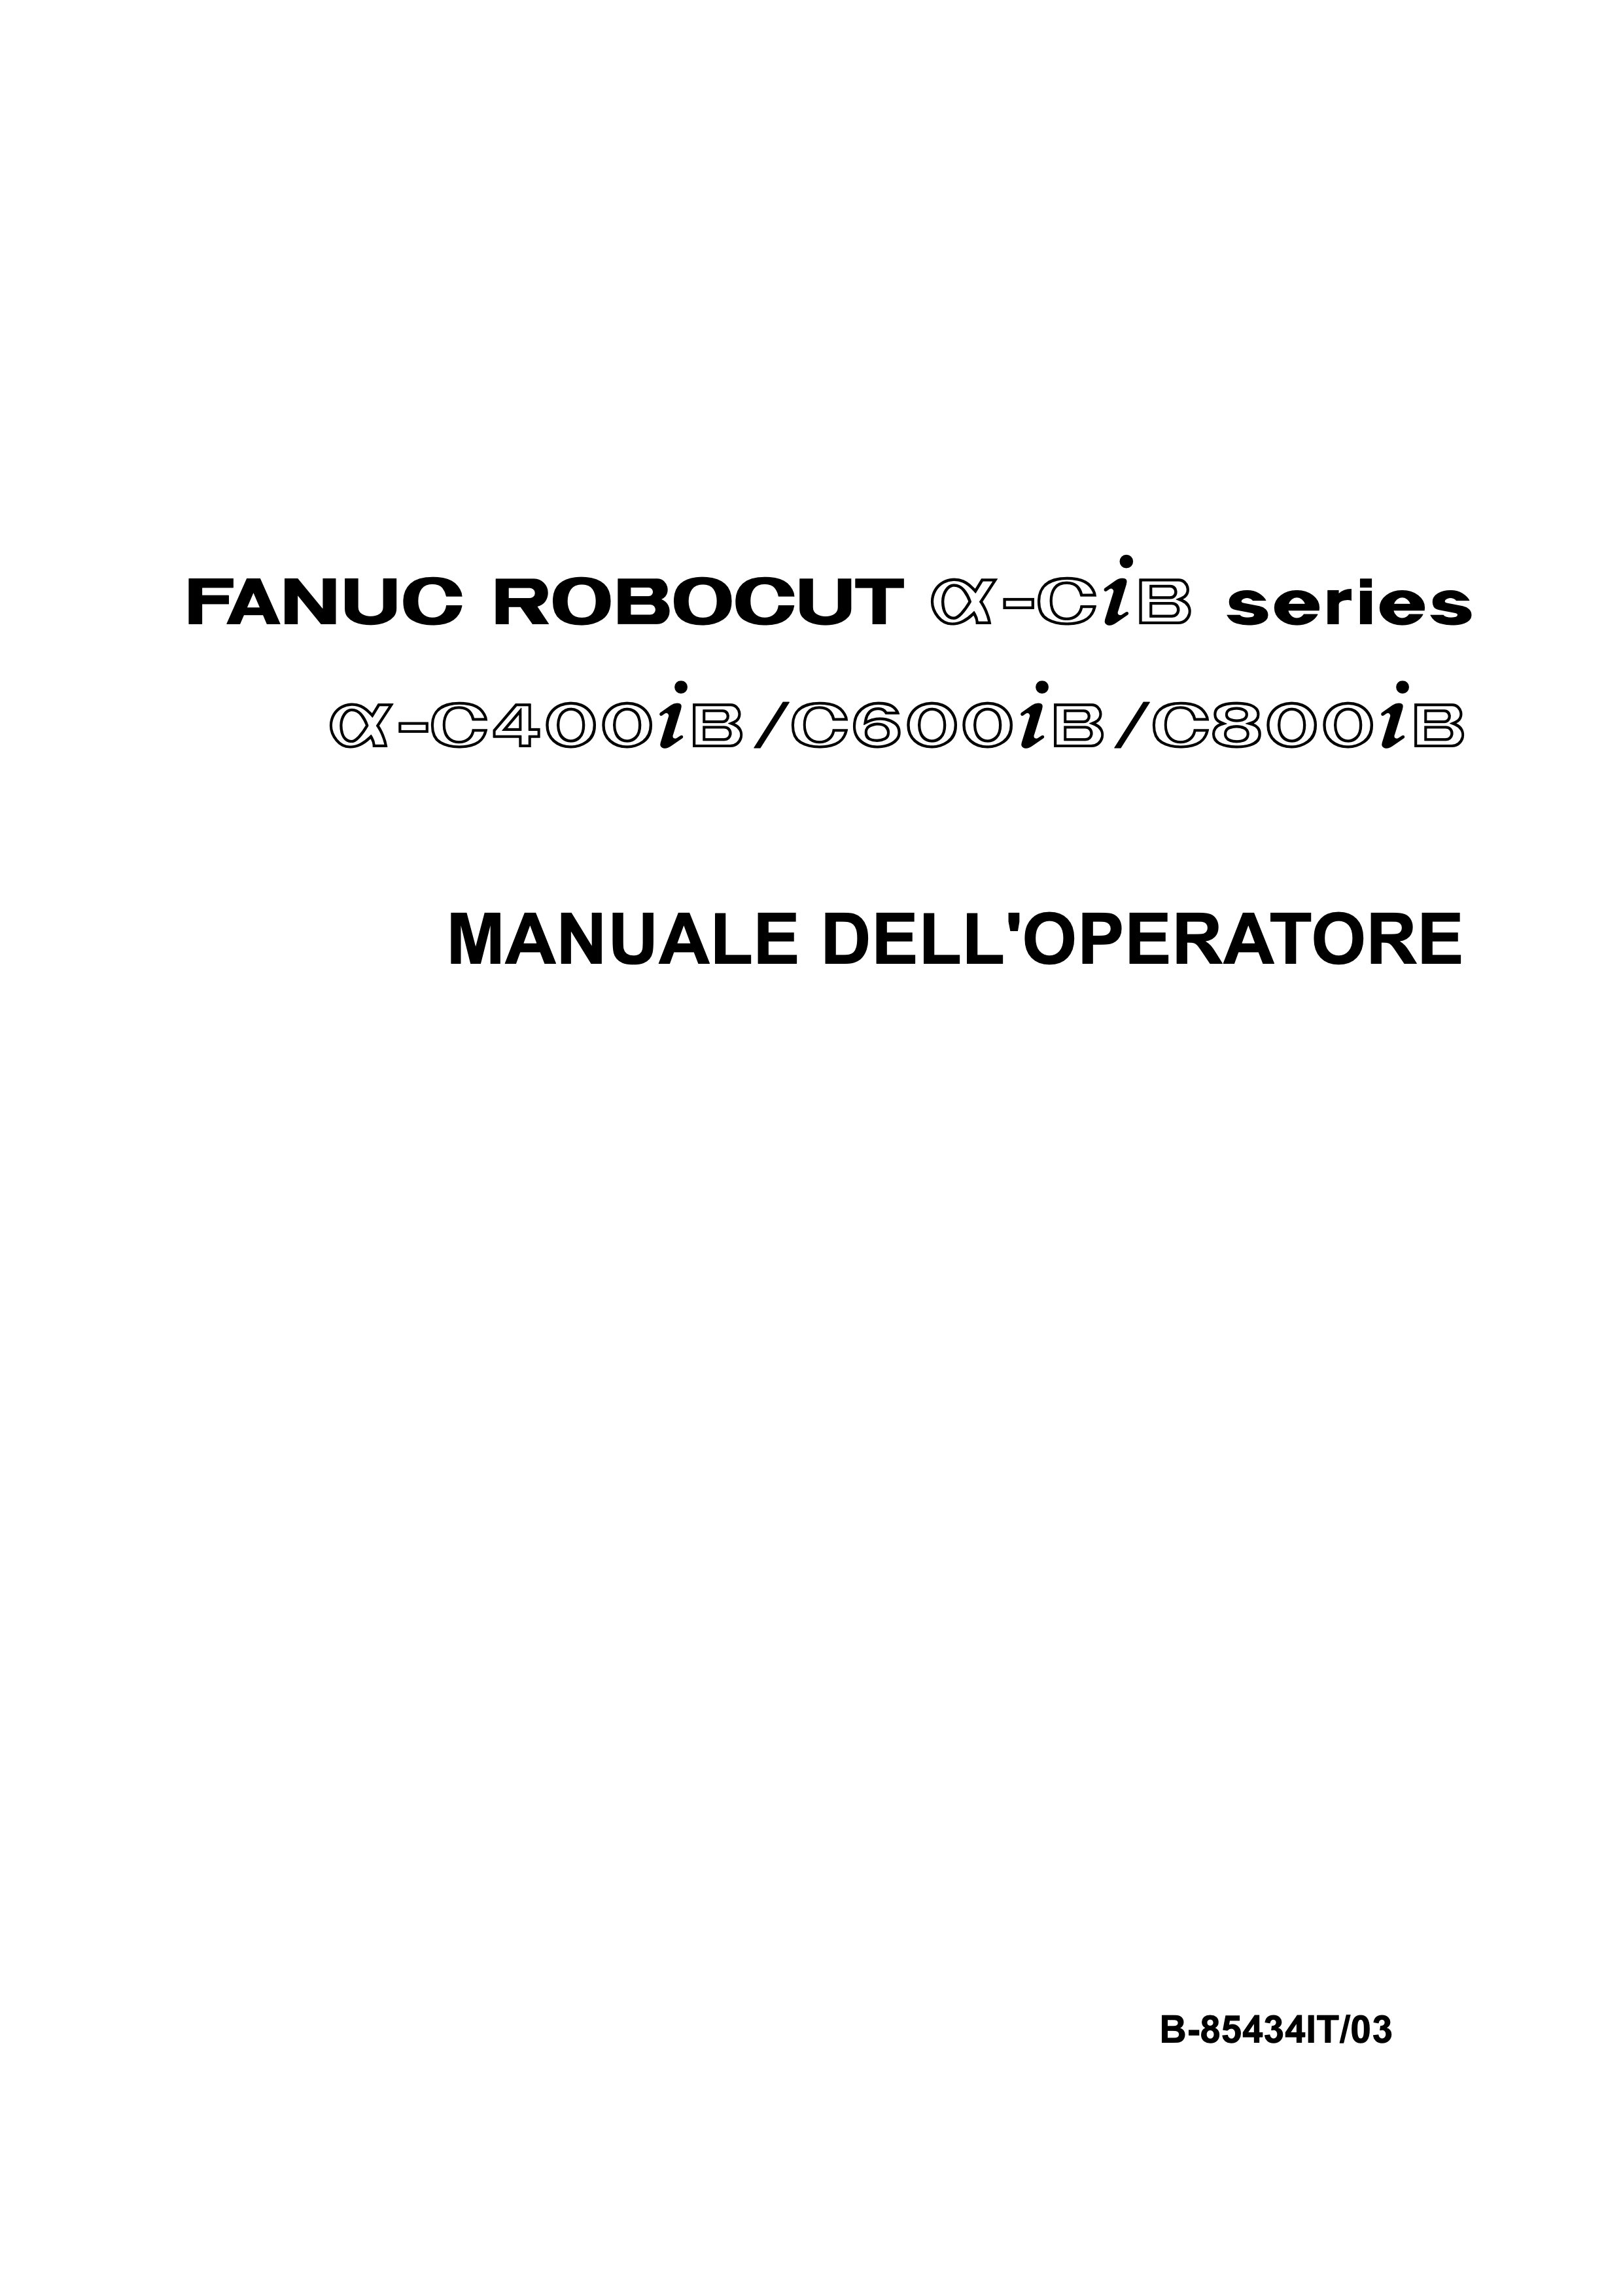
\includegraphics[height=1.95cm]{figure/asset/copertina-manuale-fanuc.png}};
\pic[scale=0.8] at (13,-5.45) {pagina};
\node[schema etichetta] at (11.7,-6.95) {Testo, figure e tabelle nel PDF};
\draw[schema freccia] (3.3,-7.4) -- (3.3,-7.95) -- (6.2,-7.95) -- (6.2,-8.5);
\draw[schema freccia] (11.7,-7.4) -- (11.7,-7.95) -- (8.8,-7.95) -- (8.8,-8.5);
\path[schema pannello,fill=schemaGrigio!5] (4.65,-13) rectangle (10.35,-8.5);
\draw[schemaGrigio] (4.65,-8.92) -- (10.35,-8.92);
\foreach \posizione/\colore in {4.95/schemaOcra,5.2/schemaVerde,5.45/schemaBlu} {\fill[\colore] (\posizione,-8.72) circle (0.05);}
\node[schema etichetta] at (7.75,-8.73) {Digital Twin nel browser};
\node[inner sep=0pt] at (7.5,-10.95) {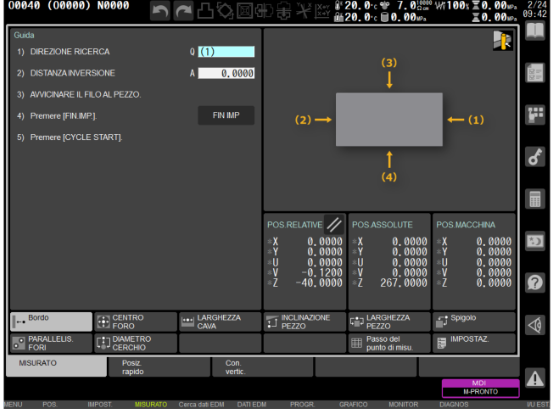
\includegraphics[width=5.15cm,height=3.85cm,keepaspectratio]{figure/asset/digital-twin.png}};
\draw[schema icona] (7.15,-13) -- (7.15,-13.25) -- (7.85,-13.25) -- (7.85,-13);
\draw[schema icona] (6.7,-13.28) -- (8.3,-13.28);
\node at (1.75,-10.4) {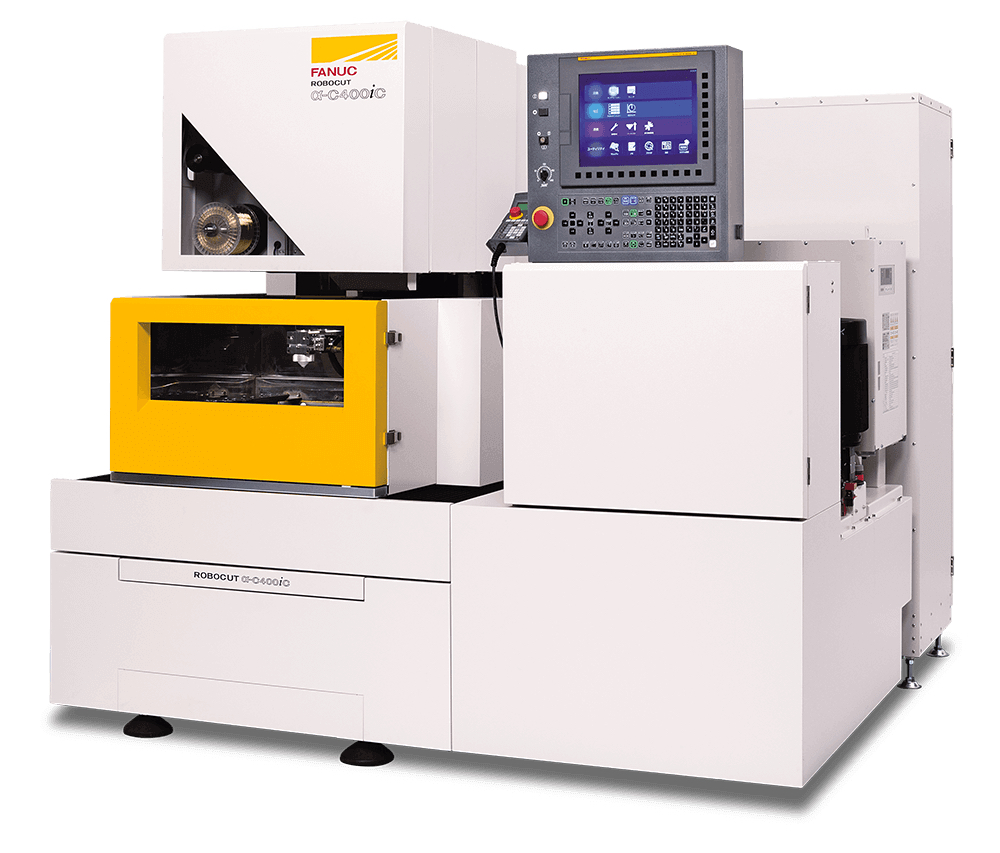
\includegraphics[width=2.85cm]{figure/asset/fanuc-robocut-c600ic-foto.jpeg}};
\node[schema nota,text width=3.35cm] at (1.75,-12.3) {Macchina di riferimento:\\la prova è in simulazione};
\draw[schema legame] (3.25,-10.4) -- (4.6,-10.4);
\node[inner sep=0pt] (operatore) at (13.15,-10.4) {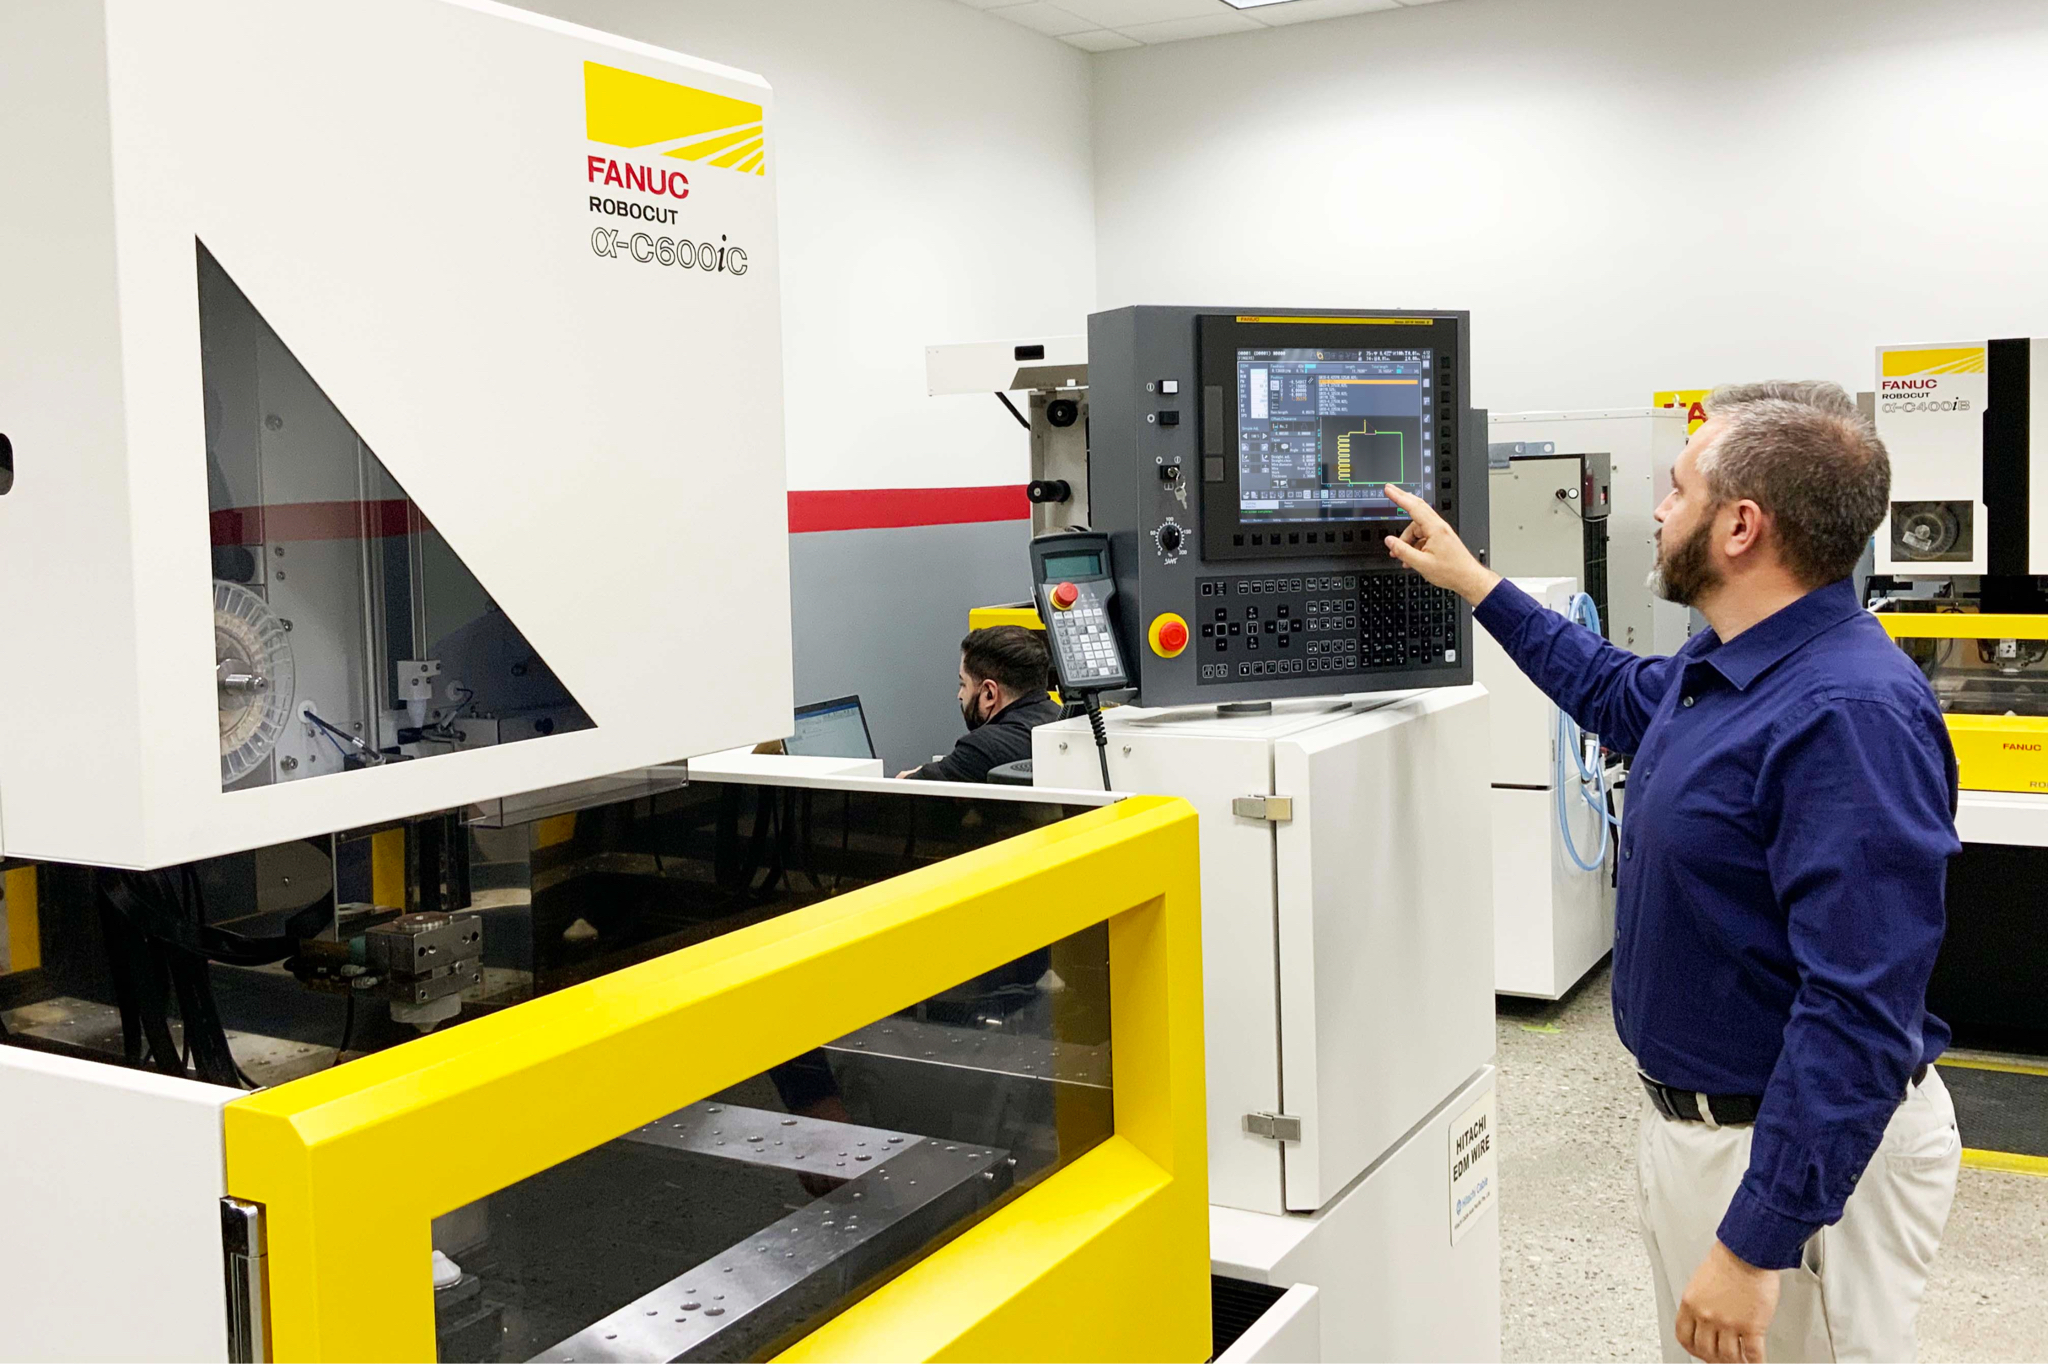
\includegraphics[width=3.6cm,height=3.85cm,keepaspectratio]{figure/asset/touch-panel-interazione-operatore.jpeg}};
\node[schema nota,text width=3.6cm,below=2mm of operatore] {L'operatore\\usa il supporto\\per individuare\\i comandi\\e svolgere il compito.};
\node[schema titolo] at (0,-14.05) {Dimensioni osservate, non risultati};
\draw[schema freccia] (7.5,-13.35) -- (7.5,-14.3);
\pic[scale=0.6] at (1.8,-15.15) {cronometro};
\pic[scale=0.6] at (5.4,-15.15) {checklist};
\path[draw=schemaOcra,fill=schemaCartaGialla,line width=1pt] (8.5,-15.5) -- (9,-14.6) -- (9.5,-15.5) -- cycle;
\node at (9,-15.24) {!};
\pic[scale=0.6] at (12.8,-15.15) {testo};
\node[schema etichetta] at (1.8,-16.1) {Tempi};
\node[schema etichetta] at (5.4,-16.1) {Accuratezza};
\node[schema etichetta] at (9,-16.1) {Critical failures};
\node[schema etichetta] at (12.8,-16.1) {SUS e NASA-TLX};
\end{tikzpicture}
\caption[Esperimento di Di Nardo: compiti, supporti e interfaccia]{Ricostruzione del progetto di Pasquale Di Nardo a partire dallo schema sperimentale fornito dall'autore della tesi. La schermata del Digital Twin è ritagliata dalla stessa figura; macchina, copertina e immagine di interazione con il touch panel provengono dai materiali allegati. Le vignette di dialogo sono schematiche, non risposte registrate. A e B indicano condizioni dello stesso partecipante, non gruppi distinti né un ordine di esecuzione. Questa sperimentazione non è la validazione finale della pipeline.}
\label{fig:esperimento-dinardo}
\end{figure}